\section{RDMA Background} \label{background}
RDMA infrastructure is built for distributed applications that require high-performance and low latency network communications. It uses a zero copy approach to deliver data between servers. With RDMA, applications can read and write memory of a remote machine, without the participation of CPU and OS kernel on both sides.

\begin{figure}[!ht]
	\centering
	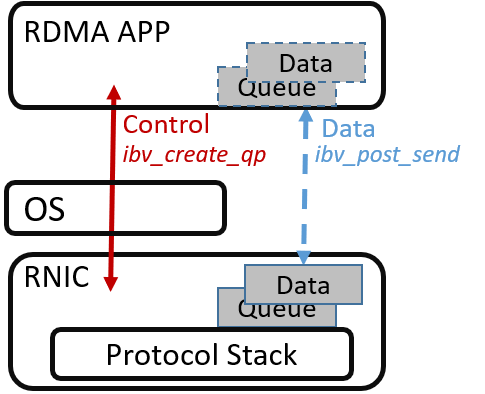
\includegraphics[width=0.75\linewidth]{images/rdma-feat.png}
	\caption{Native RDMA Architecture}
	\label{fig:rdma-feat}
\end{figure}

RDMA can be implemented in different ways, for example, InfiniBand~\cite{infiniband}, Roce~\cite{roce}, and iWARP~\cite{iwarp}.
OpenFabrics Enterprise Distribution~(OFED~\cite{ofed-manual}) is a widely used RDMA software stack that builds an abstraction layer to hide the differences of underneath drivers and hardware.
OFED stack consists of the user-space part and the kernel-space part.
As shown in Figure~\ref{fig:rdma-feat}, in user-space, RDMA applications use Verbs APIs~(also known as IB Verbs~\cite{verbs}) to send and receive data. It is similar to socket layer for traditional network applications. On the control path, Verbs provides APIs like \texttt{ibv\_create\_qp} and \texttt{ibv\_reg\_mr}. On the data path, Verbs provides APIs like \texttt{ibv\_post\_send} and \texttt{ibv\_post\_recv}. On the control path, the Verbs library forwards requests to OFED core in OS kernel. Device specific drivers that control the RDMA hardware are registered in OFED core. On the data path, the OS kernel is bypassed. So the Verbs library calls device specific user level library to send and receive data.

In the workflow of RDMA, the control path and the data path are separated. As shown in Figure~\ref{fig:rdma-feat}, on the control path, the application explicitly creates QP~(Queue Pair), CQ~(Completed Queue), registers MR~(Memory Region) and other RDMA metadata, and caches the metadata to RNIC, such as queue ID, MR key and page tables. On the data path, the application can write to the DoorBell register to notify RNIC of a new request. RNIC will read the request in the QP, read/write the contents of the local/remote MR, and put the completion notifications into the CQ. The application can poll the CQ to get the notifications. The housekeeping work is done on the control path that involves the OS kernel. The performance critical data transmission work on the data path totally bypasses the OS kernel.